\section{Auswertung}
\label{sec:Auswertung}

\subsection{Messung bis 1 bar}

  Um die gemittelte Verdampfungswärme $L$ zu bestimmen, wird zunächst der
  Logartithmus des Dampfdrucks gegen die reziproke absolute Temperatur
  dargestellt und dann die gesuchte Größe mittels einer Ausgleichsrechnung
  bestimmt. \\
  Diese Relation ergibt sich aus Formel \ref{eqn:druck2}. Diese wird weiter umgestellt zu:
  \begin{align}
    \label{eqn:druck3}
    \ln\left(\frac{p}{p_0}\right)=- \frac{L}{R} \frac{1}{T}
  \end{align}
  \\
  Wobei $p_0$ der zu Beginn gemessene Umgebungsdruck $p_0 = 994 \cdot \, \mathrm{10^2 Pa}$ ist.
  \\
  Die verwendeten Messwerte für \autoref{fig:plot1} lassen sich in \autoref{tab:bis1} finden.
  \\
  \begin{figure}
    \centering
    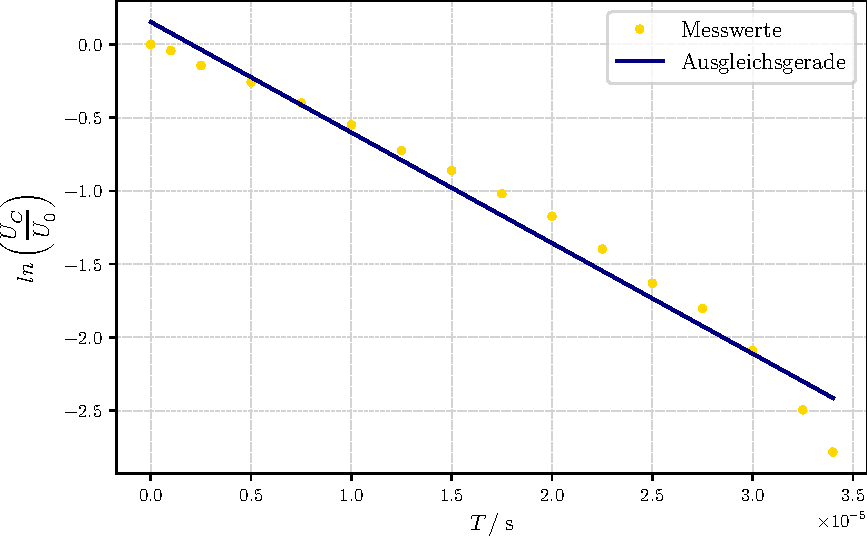
\includegraphics{plot1.pdf}
    \caption{Ausgleichsgerade für <1 bar}
    \label{fig:plot1}
  \end{figure}

  Die Ausgleichsgerade hat die Form $\ln(\frac{p}{p_0}) = m \frac{1}{T}+b$, wobei

  \begin{align*}
    m &= (-3,96 \pm 0,05) \cdot \, \mathrm{10^3 \cdot K \, \,\, und} \\
    b &= (10,73 \pm 0,16) \, \mathrm{ist.}
  \end{align*}

  Die Messunsicherheit wurde mit Python berechnet.\\
  Es wird nun die Formel der Ausgleichgerade mit Formel \ref{eqn:druck3} verglichen und
  festgestellt, dass $m=-\frac{L}{R}$ gilt. Durch Umformen erhät man folgende Formel:
  \begin{equation}
    L = - m \cdot R
  \end{equation}
  Einsetzen ergibt dann: $L = 32,92 \pm 0,43 \cdot 10^3 \, \mathrm{\frac{J}{mol}}.$ \\
  $R$ ist hier die Gaskonstante mit $R=8,314 \, J \cdot mol^{-1} \cdot K^{-1}$\\
  \\
  Als nächstes wird nun die äußere Verdampfungswärme $L_a$ mithilfe der Allgemeinen
  Gasgleichung (\ref{eqn:idealeGasgl}) für T$=373$K geschätzt. Die äußere Verdampfungswärme
  ist diejenige Energie, die benötigt wird, um ein Volumen $V_F$ an Wasser auf $V_D$ auszudehnen
  und ergibt sich mit (\ref{eqn:idealeGasgl}) folgendermaßen:
  \begin{align}
    L_a = p\cdot V &= R \cdot T \\
    &= 3,101 \cdot 10^3 \mathrm{\frac{J}{mol}}
  \end{align}
  Mit $L_i = L - L_a$ ergibt sich dann die innere Verdampfungswärme zu $L_i = 29,82 \pm 0,43 \cdot 10^3 \mathrm{\frac{J}{mol}}$.
  $L_i$ ist diejenige innere Energie, die das System benötigt um die molekularen Bindungskräfte zu überwinden. \\
  Um nun die innere Energie pro Molekül zu erhalten, wird das Ergebnis für die innere Energie $L_i$ durch die Avogadrokonstante $N_A$
  geteilt:
  \begin{align}
    L_{i,m} = 0,309 \pm 0,005 \, \mathrm{eV}
  \end{align}

  \begin{longtable}{c  c  c  c}
    \caption{Messwerte bis 1 bar \si{\bar}} \label{tab:bis1} \\
    \hline \multicolumn{1}{c}{\textbf{$T_{Dampf} \,/\, \mathrm{C^{\circ}}$}} & \multicolumn{1}{c}{\textbf{$T_{Dampf} \,/\, \mathrm{K}$}} & \multicolumn{1}{c}{\textbf{$p \,/\, \mathrm{mbar}$}} & \multicolumn{1}{c}{\textbf{$p \,/\, \mathrm{10^2 \, Pa}$}} \\ \hline \\
    \endfirsthead
    \multicolumn{4}{c}
    {{\bfseries \tablename\ \thetable{} -- weitergeführt von vorheriger Seite}} \\
    \hline \multicolumn{1}{c}{\textbf{$T_{Dampf} \,/\, \mathrm{C^{\circ}}$}} & \multicolumn{1}{c}{\textbf{$T_{Dampf} \,/\, \mathrm{K}$}} & \multicolumn{1}{c}{\textbf{$p \,/\, \mathrm{mbar}$}} & \multicolumn{1}{c}{\textbf{$p \,/\, \mathrm{10^2 \, Pa}$}} \\ \hline \\
    \endhead
    \endfoot
    \hline \hline
    \endlastfoot
      17  & 290,15 & 35 & 35   \\
      19  & 292,15 & 45 & 45   \\
      20  & 293,15 & 55 & 55   \\
      21  & 294,15 & 61 & 61   \\
      22  & 295,15 & 65 & 65   \\
      23  & 296,15 & 68 & 68   \\
      24  & 297,15 & 74 & 74   \\
      25  & 298,15 & 78 & 78   \\
      26  & 299,15 & 81 & 81   \\
      27  & 300,15 & 85 & 85   \\
      28  & 301,15 & 90 & 90   \\
      29  & 302,15 & 95 & 95   \\
      30  & 303,15 & 99 & 99   \\
      31  & 304,15 & 104 & 104  \\
      32  & 305,15 & 107 & 107  \\
      33  & 306,15 & 111 & 111  \\
      34  & 307,15 & 118 & 118  \\
      35  & 308,15 & 122 & 122  \\
      36  & 309,15 & 127 & 127  \\
      37  & 310,15 & 133 & 133  \\
      38  & 311,15 & 137 & 137  \\
      39  & 312,15 & 144 & 144  \\
      40  & 313,15 & 150 & 150  \\
      41  & 314,15 & 153 & 153  \\
      42  & 315,15 & 160 & 160  \\
      43  & 316,15 & 166 & 166  \\
      44  & 317,15 & 175 & 175  \\
      45  & 318,15 & 184 & 184  \\
      46  & 319,15 & 190 & 190  \\
      47  & 320,15 & 194 & 194  \\
      48  & 321,15 & 199 & 199  \\
      49  & 322,15 & 208 & 208  \\
      50  & 323,15 & 217 & 217  \\
      51  & 324,15 & 226 & 226  \\
      52  & 325,15 & 232 & 232  \\
      53  & 326,15 & 240 & 240  \\
      54  & 327,15 & 252 & 252  \\
      55  & 328,15 & 260 & 260  \\
      56  & 329,15 & 269 & 269  \\
      57  & 330,15 & 278 & 278  \\
      58  & 331,15 & 290 & 290  \\
      59  & 332,15 & 305 & 305  \\
      60  & 333,15 & 324 & 324  \\
      61  & 334,15 & 339 & 339  \\
      62  & 335,15 & 360 & 360  \\
      63  & 336,15 & 378 & 378  \\
      64  & 337,15 & 399 & 399  \\
      65  & 338,15 & 437 & 437  \\
      66  & 339,15 & 450 & 450  \\
      67  & 340,15 & 463 & 463  \\
      68  & 341,15 & 481 & 481  \\
      69  & 342,15 & 485 & 485  \\
      70  & 343,15 & 496 & 496  \\
      71  & 344,15 & 521 & 521  \\
      72  & 345,15 & 528 & 528  \\
      73  & 346,15 & 542 & 542  \\
      74  & 347,15 & 551 & 551  \\
      75  & 348,15 & 569 & 569  \\
      76  & 349,15 & 582 & 582  \\
      77  & 350,15 & 603 & 603  \\
      78  & 351,15 & 617 & 617  \\
      79  & 352,15 & 640 & 640  \\
      80  & 353,15 & 647 & 647  \\
      81  & 354,15 & 663 & 663  \\
      82  & 355,15 & 678 & 678  \\
      83  & 356,15 & 688 & 688  \\
      84  & 357,15 & 711 & 711  \\
      85  & 358,15 & 722 & 722  \\
      86  & 359,15 & 730 & 730  \\
      87  & 360,15 & 736 & 736  \\
      88  & 361,15 & 753 & 753  \\
      89  & 362,15 & 765 & 765  \\
      90  & 363,15 & 770 & 770  \\
      91  & 364,15 & 778 & 778  \\
      92  & 365,15 & 790 & 790  \\
      93  & 366,15 & 793 & 793  \\
      94  & 367,15 & 811 & 811  \\
      95  & 368,15 & 816 & 816  \\
      96  & 369,15 & 825 & 825  \\
      97  & 370,15 & 830 & 830  \\
      98  & 371,15 & 836 & 836  \\
      99  & 372,15 & 837 & 837  \\ \\
  \end{longtable} 

\subsection{Messung von 1 bis 15 bar}

Mit den Messungen von 1 bis 15 bar wird nun die Abhängigkeit der Verdampfungswärme
zu der Temperatur untersucht. Dafür wird zunächst die Clausius-Clapeyronsche Gleichung \ref{eqn:ClausiusClap}
nach L aufgelöst:

\begin{align}
  (V_D - V_F)dp = \frac{L}{T}dT \\
  \Leftrightarrow L = T(V_D - V_F)\frac{dp}{dT}
\end{align}

Um $\frac{dp}{dT}$ zu bestimmen, wird nun aus den Wertepaaren in \autoref{tab:ueber15bar} ein Ausgleichspolynom
vom 3ten Grad bestimmt und nach T abgeleitet. $V_D$ kann bei diesem Druck nicht mehr aus der Allgemeinen Gasgleichung
bestimmt werden, stattdessen wird
\begin{align}
  \left(p+\frac{a}{V^2}\right)V = RT \, \, \mathrm{mit} \, \, a = 0,9 \mathrm{\frac{J \cdot m^3}{Mol^2}} \\
  \Leftrightarrow V_D = \frac{RT}{2p} \pm \sqrt{\frac{R^2T^2}{4p^2}-\frac{a}{p}}
\end{align}
verwendet.

Damit ergibt sich:
\begin{align}
  \label{yay}
  L = \frac{T}{p} \left(\frac{RT}{2} \pm \sqrt{\frac{R^2T^2}{4}-ap}\right)\frac{dp}{dT}
\end{align}

Nun wird ein Ausgleichspolynom 3ten Grades bestimmt:
\begin{figure}
  \centering
  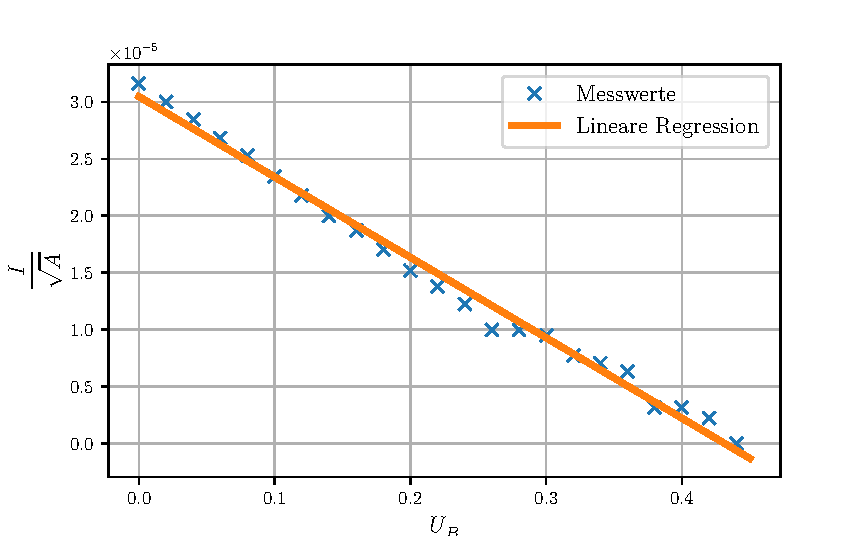
\includegraphics{plot2.pdf}
  \caption{Ausgleichspolynom 3ten Grades}
  \label{fig:plot2}
\end{figure}

das Polynom 3ten Grades besitzt die Form $p(T)= A \cdot T^3 + b \cdot T^2 + c \cdot T + d$ mit 
\begin{align*}
  A &= (1,166 \pm 0,22) \, \mathrm{\frac{Pa}{K^3}} \\
  b &= (-13,29 \pm 2,85) \cdot 10^2 \, \mathrm{\frac{Pa}{K^2}}\\
  c &= (5,12 \pm 1,23) \cdot 10^5 \, \mathrm{\frac{Pa}{K}}\\
  d &= (-6,64 \pm 1,76) \cdot 10^7 \, \mathrm{Pa}\\
  \frac{dp}{dT}= 3A \cdot T^2 + 2b \cdot T + c
\end{align*}

$p(T)$ und $\frac{dp}{dT}$ werden nun in Formel \ref{yay} eingesetzt:

\begin{align*}
L = \frac{3A \cdot T^3 + 2b \cdot T^2 + cT}{A \cdot T^3 + b \cdot T^2 + c \cdot T + d} \left(\frac{RT}{2} \pm \sqrt{\frac{R^2T^2}{4}-a\cdot(A \cdot T^3 + b \cdot T^2 + c \cdot T + d)}\right)
\end{align*}

\begin{figure}
  \centering
  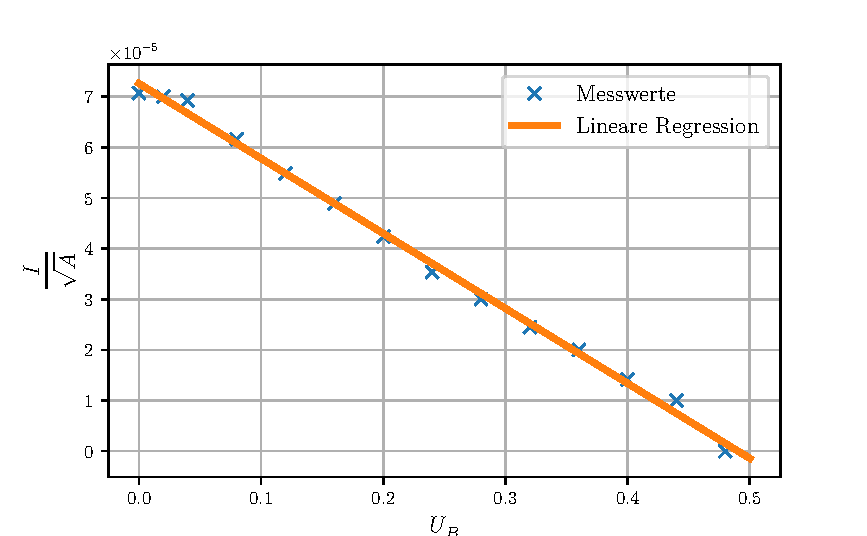
\includegraphics{plot3.pdf}
  \caption{Genäherte Funktion für L für das addieren der Wurzel}
  \label{fig:plot3}
\end{figure}

\begin{figure}
  \centering
  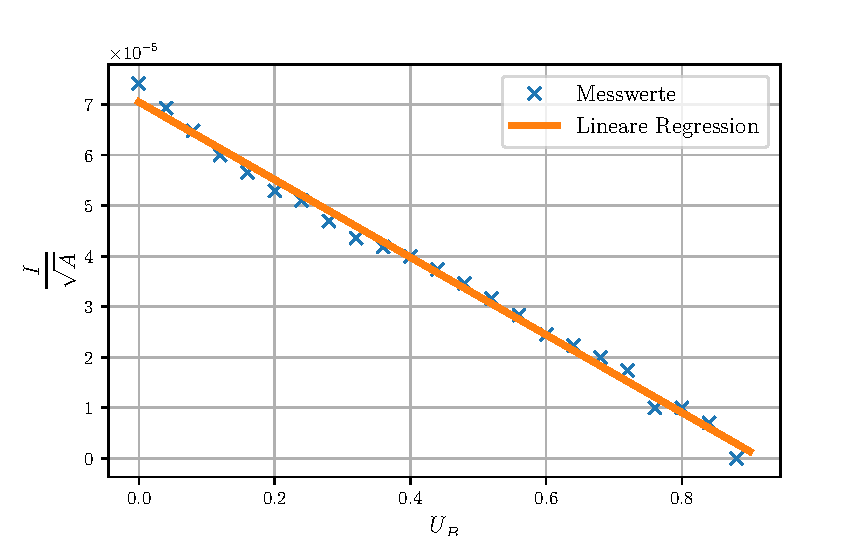
\includegraphics{plot4.pdf}
  \caption{Genäherte Funktion für L für das subtrahieren der Wurzel}
  \label{fig:plot4}
\end{figure}


\begin{longtable}{c  c}
  \caption{Messwerte 1 bis 15 \si{\bar}} \label{tab:ueber15bar} \\
  \hline \multicolumn{1}{c}{\textbf{$T \,/\, \mathrm{C^{\circ}}$}} & \multicolumn{1}{c}{\textbf{$p \,/\, \mathrm{bar}$}} \\ \hline \\
  \endfirsthead
  \multicolumn{2}{c}
  {{\bfseries \tablename\ \thetable{} -- weitergeführt von vorheriger Seite}} \\
  \hline \multicolumn{1}{c}{\textbf{$T_{Dampf} \,/\, \mathrm{C^{\circ}}$}} & \multicolumn{1}{c}{\textbf{$p \,/\, \mathrm{bar}$}} \\ \hline \\
  \endhead
  \endfoot
  \hline \hline
  \endlastfoot

  117 & 1 \\
  132 & 2 \\
  141 & 3 \\
  150 & 4 \\
  158 & 5 \\
  163 & 6 \\
  169 & 7 \\
  174 & 8 \\
  178 & 9 \\
  182 & 10 \\
  186 & 11 \\
  189 & 12 \\
  193 & 13 \\
  196 & 14 \\
  198 & 15 \\ \\
\end{longtable} 



